\documentclass{article}
\usepackage[english, russian]{babel}
\usepackage{import}
\usepackage[utf8]{inputenc}
\usepackage{graphicx} % Required for inserting images
\usepackage{multicol}
\usepackage{enumitem}
\usepackage[square]{natbib}
\graphicspath{ {images/} }
\usepackage[left=2cm, right=2cm, bottom=2cm, top=2cm]{geometry}
\title{\textbf{Intelligent Tutoring System
for Discrete Mathematics}}

\begin{document}

\normalsize

\begin{center}
\begin{SCfigure}
    \centering
    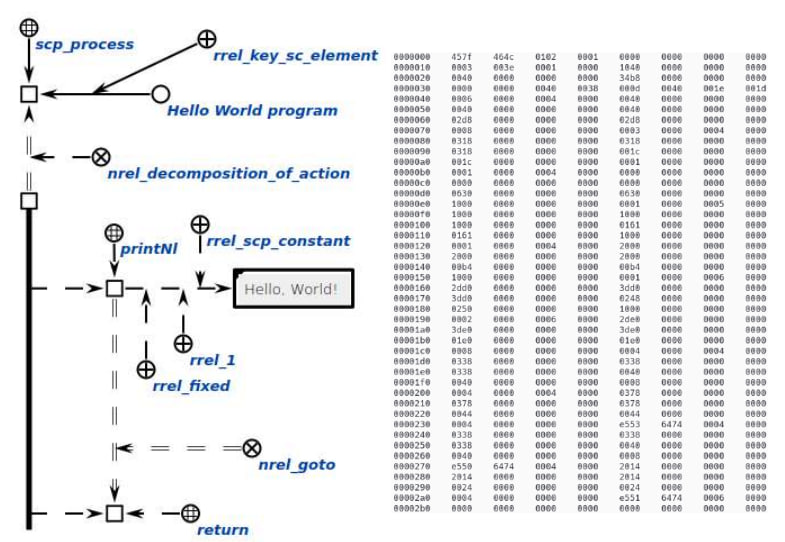
\includegraphics[width=17cm]{picture_for_laba1pivas.jpg}
    \captionsetup
    \caption{Figure 8: Example of a “Hello World” program written in SCP (left) and machine code (right)}
\end{SCfigure}
\end{center}


\begin{multicols}{2}
\renewcommand{\baselinestretch}{0.5}
An option was proposed to implement a mechanism for
differentiation of access to the knowledge bases of ostissystems based on the ABAC model. The work examined
an example of the architecture of the OSTIS Ecosystem
based on the Matrix protocol, as well as ideas for the
implementation of safety measures of a personal ostisassistant and for the agents’ source code.

\begin{center}
    References
\end{center}

\footnotesize
\begin{enumerate}[label=\text{[\arabic*]}, noitemsep,topsep=1.5pt,parsep=1.5pt,partopsep=1.5pt]
\item S. Isoboev, D. Vezarko, and A. Chechelnitsky, “Intellektual’naya
sistema monitoringa bezopasnosti seti besprovodnoi svyazi
na osnove mashinnogo obucheniya [wireless communication
network security intelligent monitoring system based on machine
learning],” \textit{Ekonomika i kachestvo sistem svyazi [Economics and
quality of communication systems]}, vol. 1, no. 23, pp. 44–48,
2022.
\item V. Chastikova and A. Mitiugov, “Metodika postroeniya sistemy
analiza intsidentov informatsionnoi bezopasnosti na osnove
neiroimmunnogo podkhoda [methodology for building a system
for analyzing information security incidents based on the
neuroimmune approach],” \textit{Elektronnyi Setevoi Politematicheskii
Zhurnal «Nauchnye Trudy Kubgtu» [Electronic Network
Polythematic Journal «Scientific Works of the KubSTU»]}, no. 1,
pp. 98–105, 2022.
\item A. Skrypnikov \tetxit{et al}., “Reshenie zadach informatsionnoi
bezopasnosti s ispol’zovaniem iskusstvennogo intellekta
[solving information security problems using artificial
intelligence],” \tetxit{Sovremennye naukoemkie tekhnologii [Modern
high technologies]}, no. 6, pp. 277–281, 2021.
\item E. Sozinova, “Primenenie ekspertnykh sistem dlya analiza
i otsenki informatsionnoi bezopasnosti [application of expert
systems for analyzing and assessing the information security],”
\tetxit{Molodoi uchenyi [Young scientist]}, vol. 10, no. 33, pp. 64–66,
2011.
\item \textit{Information security, cybersecurity and privacy protection —
Evaluation criteria for IT security — Part 1: Introduction and
general model}, ISO/IEC Std. 15 408-1, 2022.
\item V. Golenkov, Ed., \textit{Tehnologija kompleksnoj podderzhki
zhiznennogo cikla semanticheski sovmestimyh intellektual’nyh
komp’juternyh sistem novogo pokolenija [Technology of complex
life cycle support of semantically compatible intelligent computer
systems of new generation]}. Bestprint, 2023.
\item D. Abdurakhman, “Iskusstvennyi intellekt i mashinnoe obuchenie
v kiberbezopasnosti [artificial intelligence and machine learning
in cybersecurity],” \textit{Sovremennye problemy lingvistiki i metodiki
prepodavaniya russkogo yazyka v vuze i shkole [Modern problems
of linguistics and methodology of teaching Russian language at
university and school]}, no. 34, pp. 916–921, 2022.
\item Cwe view: Research concepts. Available at: https://cwe.mitre.org/
data/definitions/1000.html (accessed 2024, Feb).
\item V. Ivashenko, \textit{Modeli resheniya zadach v intellektual’nykh
sistemakh. V 2 ch. Ch. 1 : Formal’nye modeli obrabotki
informatsii i parallel’nye modeli resheniya zadach : ucheb.-metod.
posobie [Models for solving problems in intelligent systems. In
2 parts, Part 1: Formal models of information processing and
parallel models for solving problems: a tutorial]}. BGUIR, 2020.
\item V. Druzhinin and D. Ushakov, Eds., \textit{Kognitivnaya psikhologiya.
Uchebnik dlya vuzov [Cognitive psychology. Textbook for
universities]}. PER SE, 2002.
\item R. Dushkin, \textit{Metody polucheniya, predstavleniya i obrabotki
znanii s NE-faktorami [Methods of gaining, representation and
processing of knowledge with NON-factors]}, 2011.
\item A. Gribkov, “Formirovanie dostovernogo znaniya: nakhozhdenie
znanii i vyyavlenie defektov [the formation of reliable
knowledge: Finding knowledge and identifying defects],” \textit{Vestnik
Leningradskogo gosudarstvennogo universiteta imeni A. S.
Pushkina [A.S. Pushkin Leningrad State University Journal]}, pp.
74–90, 2023.
\item A. Dementev, “Metriki semanticheskikh dannykh [metrics for
semantic data],” \textit{Molodoi uchenyi [Young scientist]}, vol. 24, no.
419, pp. 48–51, 2022.
\item A. Narinyani, “Ne-faktory: Netochnost’ i nedoopredelennost’ -
razlichie i vzaimosvyaz’ (doformal’noe issledovanie) [non-factors:
Inaccuracy and under-determination - distinction and relationship
(pre-formal study)],” \textit{Mezhdunarodnyi Seminar DIALOG’99
Tarusa [International Seminar DIALOG’99 Tarusa]}, 1999.
\item I. Davydenko, “Semantic models, method and tools of knowledge bases coordinated development based on reusable components,” \textit{Otkrytye semanticheskie tehnologii proektirovanija intellektual’nyh sistem [Open semantic technologies for intelligent
systems]}, pp. 99–118, 2018.
\item A. Ostroukh, \textit{Intellektual’nye sistemy: monografiya [Intelligent
systems: monograph]}. Nauchno-innovatsionnyi tsentr, 2020.
\item A. Baranovich, “Semanticheskie aspekty informatsionnoi
bezopasnosti: kontsentratsiya znanii [semantic aspects of
information security: concentration of knowledge],” \textit{Istoriya i
arkhivy [History and Archives]}, vol. 13, no. 75, pp. 38–58, 2011.
\item Matrix specification. Available at: https://spec.matrix.org/v1.9/
(accessed 2024, Mar).
\item Openpgp. Available at: https://www.openpgp.org/ (accessed 2024,
Mar).
\item P. Cousot and R. Cousot, “Abstract interpretation: Past, present
and future,” CSL-LICS ’14: \textit{Proceedings of the Joint Meeting of
the Twenty-Third EACSL Annual Conference on Computer Science
Logic (CSL) and the Twenty-Ninth Annual ACM/IEEE Symposium
on Logic in Computer Science (LICS)}, pp. 1–10, 2014.
\item V. Khoang and A. Tuzovskii, “Resheniya osnovnykh zadach
v razrabotke programmy podderzhki bezopasnosti raboty s
semanticheskimi bazami dannykh [solutions to the main problems
in the development of a program to support the security of work
with semantic databases],” \textit{Doklady Tomskogo gosudarstvennogo
universiteta sistem upravleniya i radioelektroniki [Proceedings of
Tomsk State University of Control Systems and Radioelectronics]},
vol. 2, no. 28, pp. 121–125, 2013.
\item A. Lajevardi and M. Amini, “Big knowledge-based semantic
correlation for detecting slow and low-level advanced persistent
threats,” \textit{Journal of Big Data,} vol. 8, no. 148, 2021.
\item V. Ivashenko, N. Zotov, and M. Orlov, “Semantic logging of
repeating events in a forward branching time model,” \textit{Pattern
Recognition and Information Processing (PRIP’2021): Proceedings of the 15th International Conference}, p. 149–152, 2021.
\end{enumerate}

\columnbreak

\raggedcolumns

\begin{center} 
\renewcommand{\baselinestretch}{1.0}
\normalsize
\textbf{ПРОБЛЕМЫ БЕЗОПАСНОСТИ
ЭКОСИСТЕМЫ OSTIS}
\end{center}
\begin{center}
\normalsize
    Хорошавин В. Д., Захаров В. В.
\end{center}

\footnotesize В данной работе рассматриваются угрозы и уязвимости,
актуальные для ostis-систем. Разграничение доступа к базам
знаний остис-систем, реализация механизмов настройки
персонального остис-ассистента и безопасность исходного
кода агентов определены как основные направлениями обеспечения безопасности остис-систем. Предложены варианты
реализации соответствующих механизмов безопасности по
этим направлениям.


\begin{flushright}
    Received 13.03.2024
\end{flushright}

\end{multicols}

\newpage
\begin{center}
\Huge
    \textbf{Intelligent Tutoring System\\
for Discrete Mathematics}\\
\end{center}
\begin{center}
\small
\text{Kanstantsin Shurmel and Artur Sharapov\\
Eugene Samokval and Vitaly Tsishchanka\\
\textit{Belarusian State University of\\
Informatics and Radioelectronics}\\
Minsk, Belarus\\
Email: shurmel.konstantin@mail.ru, arturshaser@gmail.com\\
samokvalz@gmail.com, vitalik.tsishchanka@gmail.com}\\
\end{center}

\begin{multicols}
\normalsize
    \textbf{Abstract—The article presents a model of intelligent
tutoring system for discrete mathematics. The model of such
system uses methods and tools designed to build intelligent
tutoring systems for any discipline and easy integration of
new disciplines into the existing tutoring system.}\\
\indent
\textbf{\textit{Keywords}—knowledge, knowledge base, intelligent systems, problem solver, interface, discrete mathematics.}\\
\begin{center}
    I. Introduction
\end{center}

\textit{Discrete mathematics} is fundamental these days and
finds wide application in various fields. These fields
include logistics, geographic information systems, computer science, modeling of physical and mathematical
phenomena. This variety of applications makes \textit{discrete
mathematics} attractive both to commercial organizations
looking for process optimization and solving complex
problems, and to non-profit organizations engaged in research and development of new methods and algorithms.
\par 
Moreover, there are many other fields in which \tetxit{discrete
mathematics} has potential for application, such as sociology, biology, chemistry, and economics. This emphasizes
its importance and relevance in modern society. Hence,
understanding \textit{discrete mathematics} plays an important
role in the progress of science and technology. Therefore,
in order for people to learn this science in a convenient
way, it is necessary to develop new teaching methods
to make the educational material more effective and
accessible.
\par
Modern methods of tuition involve not only internal
presence of the learner in a particular discipline, but also
the possibility of distance learning. As a rule, many of
those who already have higher professional education,
wish to deepen their knowledge in the discipline of
interest, to expand competence in a related professional
field of activity and to obtain new skills and knowledge,
giving the opportunity to occupy a more successful
position in the professional environment.
\par
The first mention of the concept of \textit{intelligent tutoring
systems} was defined in 1970 by J. Carbonell. More than
10 years later, real working intelligent tutoring systems
appeared. The difference between \textit{intelligent tutoring
systems} and automated systems is that \textit{automated system}
is a \textit{consolidated knowledge base}, based on the results
of work with which the system gives the learner the
results of correctly and incorrectly answered questions.
In turn, \textit{intelligent tutoring system} is aimed at the process
of diagnosing learning, its correction. The essence of
the work of such a system is not just in diagnosing the
learner’s mistakes, but also in issuing advice based on
predetermined strategies of distance learning [1].\\
\newline
\textbf{\textit{Intelligent tutoring system}}
\begin{enumerate}
    \item [:=] [A set of software and hardware that uses \textit{artificial
intelligence} techniques to create interactive and adaptive educational tools. Such systems are usually able
to adapt to the individual needs and knowledge level
of each learner, offering personalized assignments,
materials selection and feedback.]
\end{enumerate} \\
\newline
\textbf{\textit{Automated learning system}}
\begin{enumerate}
    \item [:=] [A program or set of programs that facilitate or fully
automate the learning process. They may include
various functions such as organizing learning material, creating tests and assignments, and tracking
student progress. Such systems are usually designed
to optimize the learning process, reduce the time
spent on routine teacher tasks, and improve learning
efficiency.]
\end{enumerate} \\

\par
\textbf{The main advantages of an intelligent tutoring
system:}


\begin{itemize}[noitemsep,topsep=1pt,parsep=1pt,partopsep=1pt]
    \item personalized approach to learning, taking into account the individual needs and knowledge level of
each student;
\item the possibility of interactive classes and the use of
visualization to explain theoretical concepts more
clearly;
\item automatic identification of students’ weaknesses and
suggestion of additional materials to reinforce the
material;
\item providing access to a wide range of educational
\end{itemize}
    

\end{multicols}


\end{document}
